\clearpage
\section{The build}
\subsection{Power supply}
After consulting a fellow student from the Electrical Engineering faculty, we acquired a power adapter able to provide enough amperes(hopefully) to run the entire cluster. After ordering some USB heads from Ebay we set out to create our own high powered USB hub. 

The Lacie power adapter comes with a 4 pin connector providing 12V and 5V. Since only the 5V is needed, we cut the cable and put on a new connector jack connecting only the 5V and ground. This also provided us with an easy way to remove the cable for when we need to turn off or move the cluster. 

Once we had a power source we set up a simple circuit with only one USB head to test. After measuring and making sure everything was in order a Raspberry PI was connected. It booted and everything was working, so our proof of concept was done.  

Next came building the USB hub. 8 USB connectors were soldered to a prototyping PCB along with the female part of the connector jack providing the power. Everything was connected in parallel using the twisted pair cables salvaged from an Ethernet cable.  

\begin{figure}[h]
	\centering
    \includegraphics[width=0.5\textwidth]{thebuild/result.png}
    \caption{Power supply: end result}
    \label{fig:build_power_supply}
\end{figure}

\subsection{The cluster}
sample text

\begin{figure}[h]
	\centering
    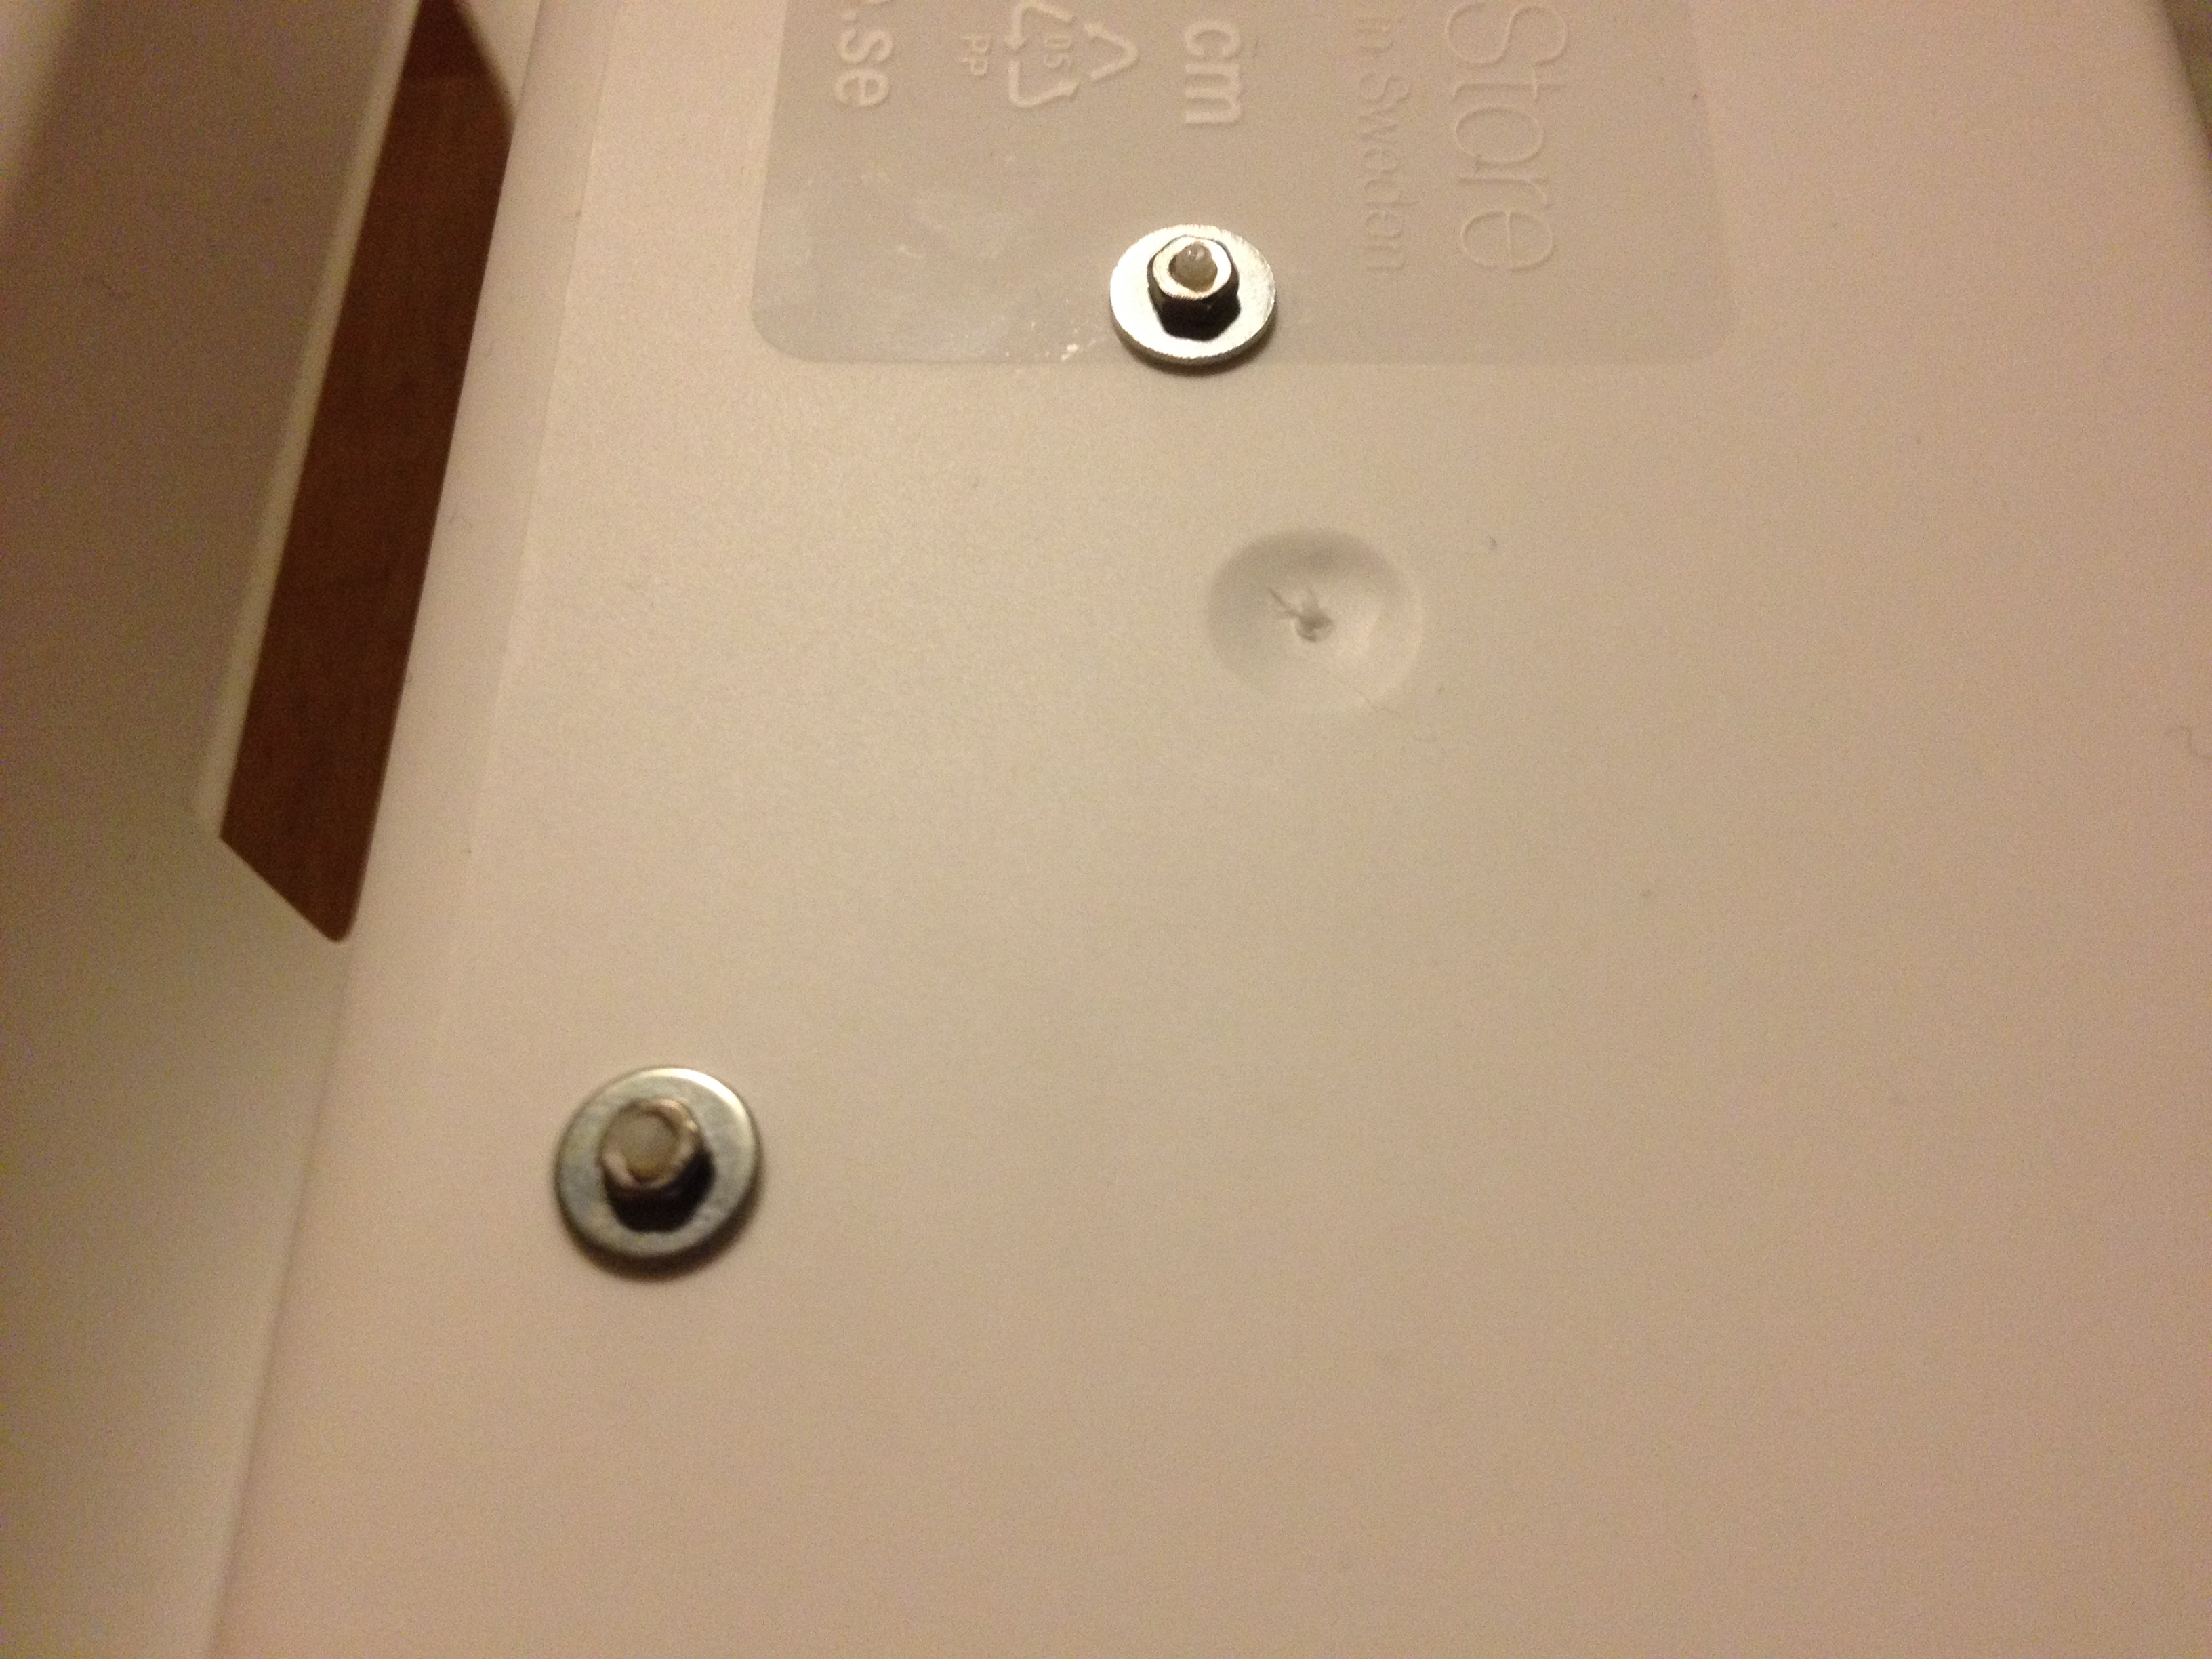
\includegraphics[width=0.5\textwidth]{thebuild/cluster_under.jpg}
    \caption{Under the clusterbox}
    \label{fig:build_cluster_under}
\end{figure}

\begin{figure}[h]
	\centering
    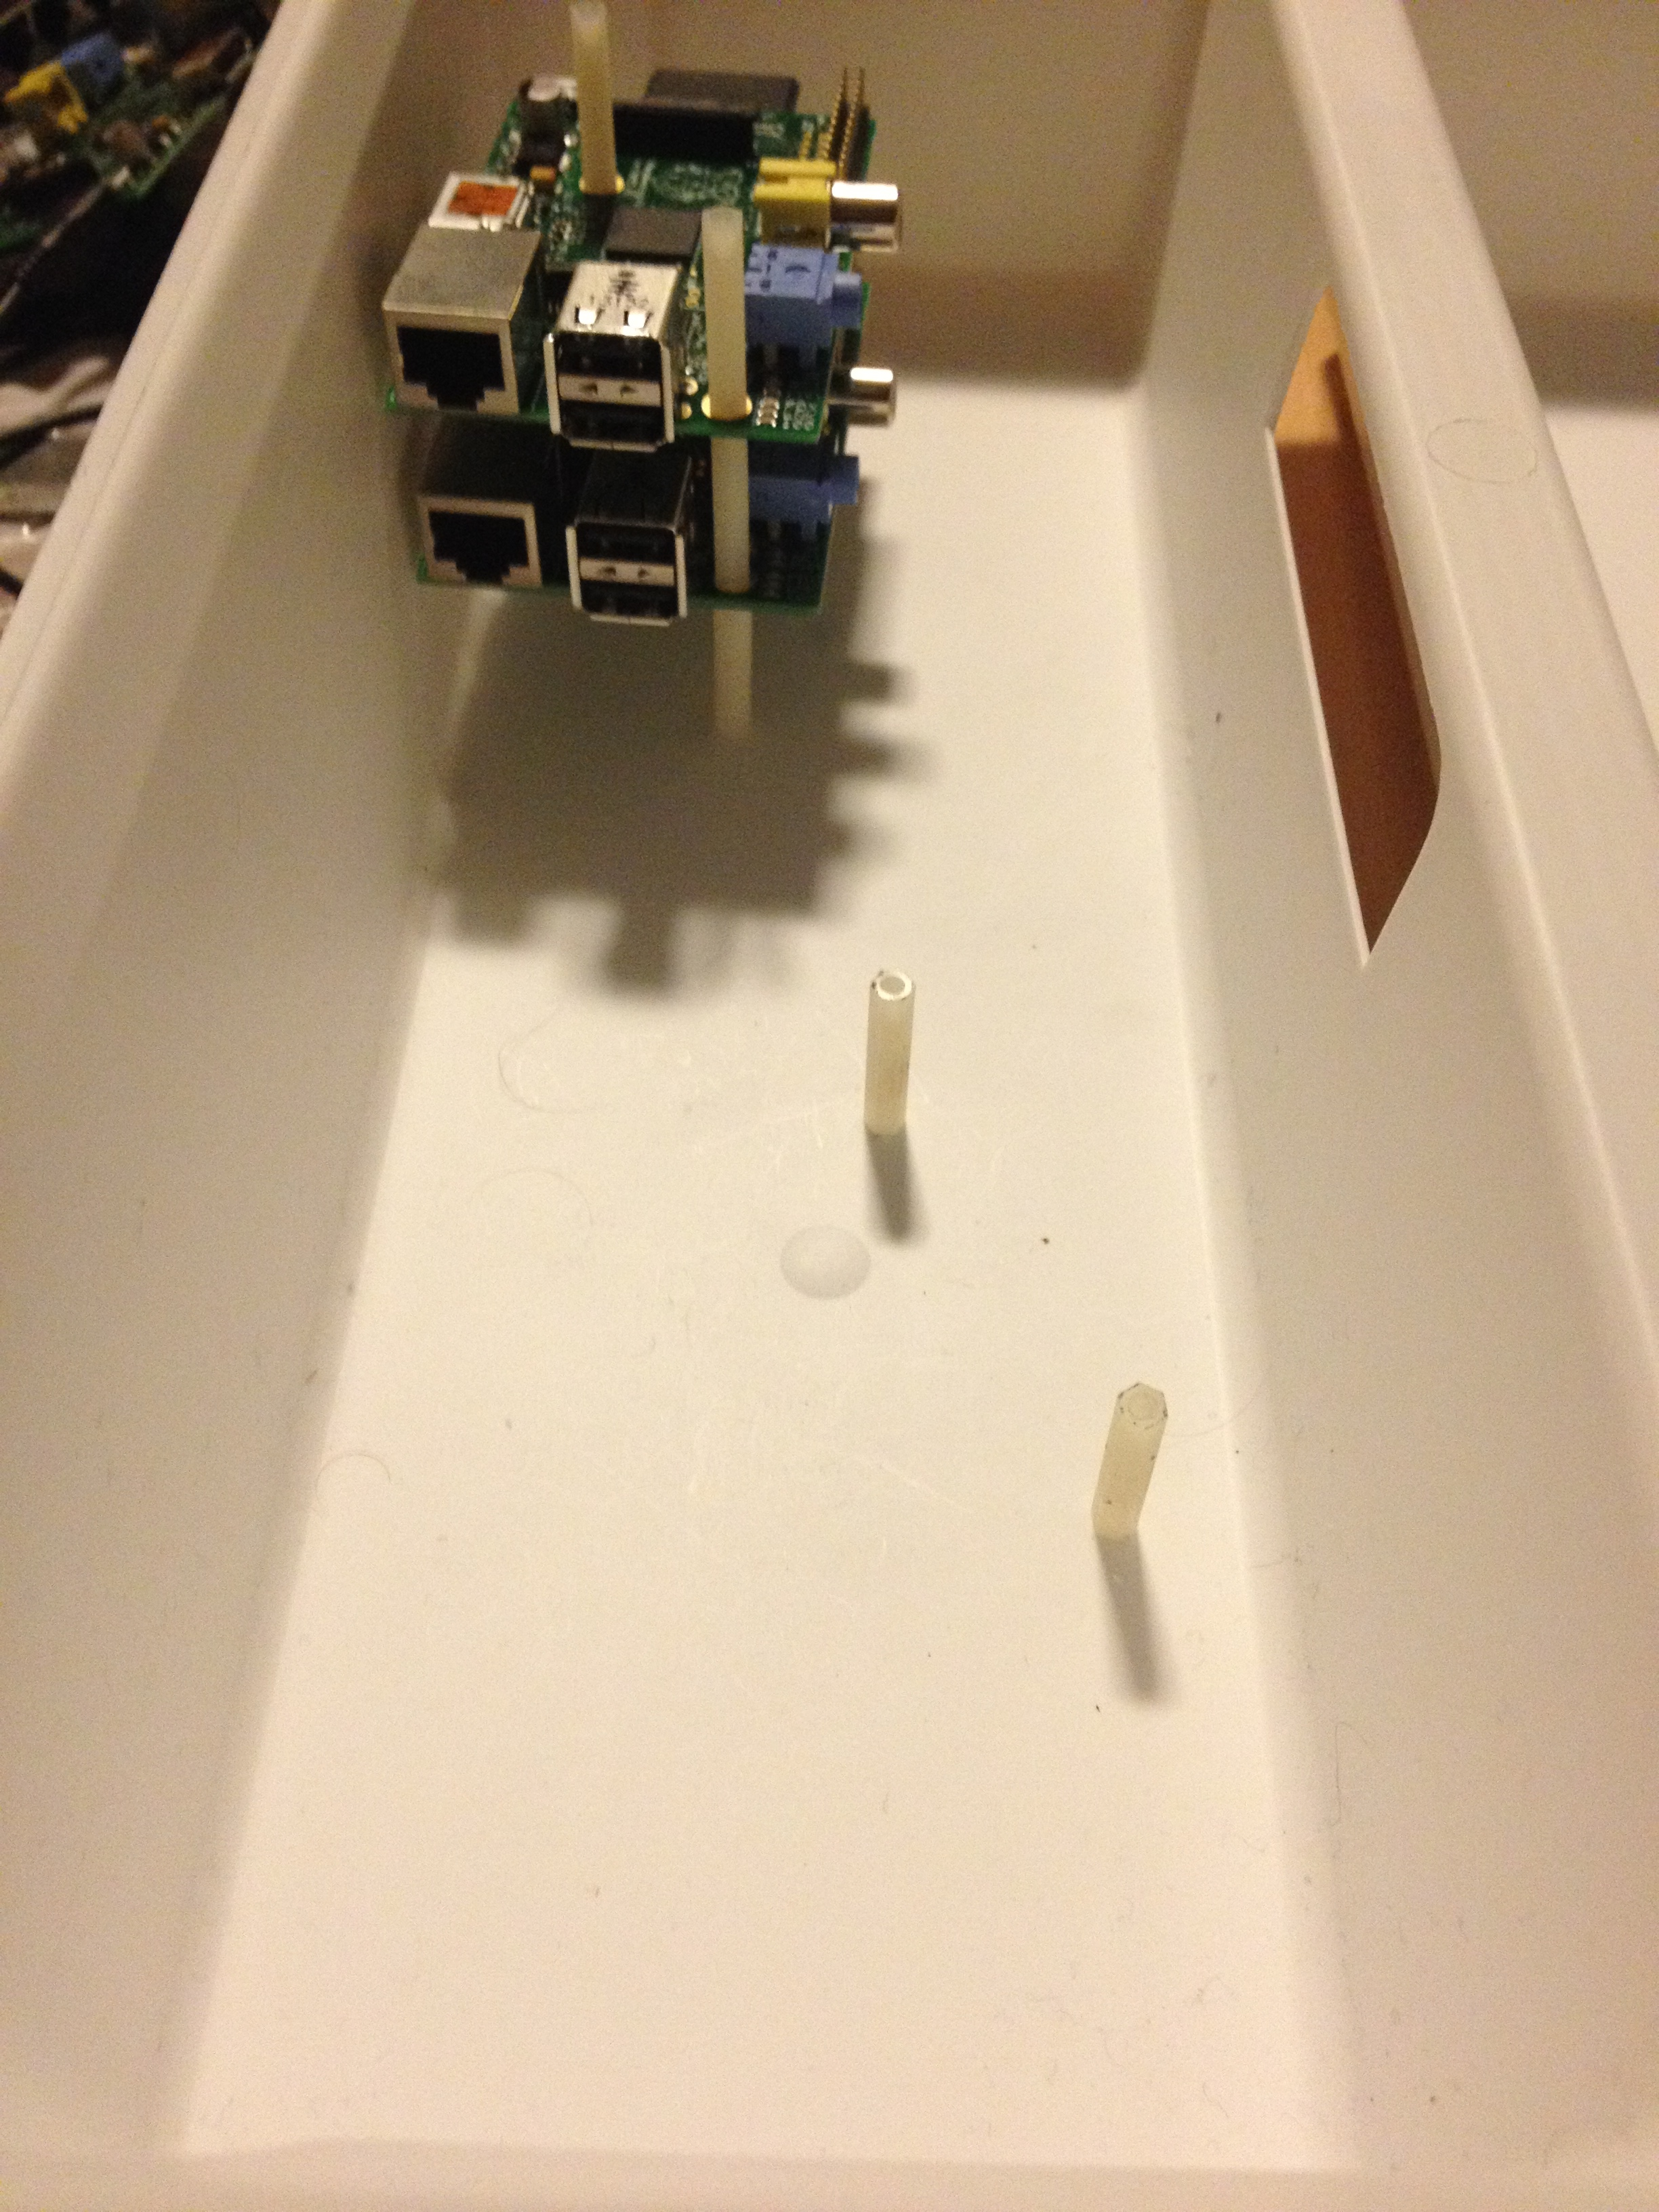
\includegraphics[width=0.5\textwidth]{thebuild/cluster_inside.jpg}
    \caption{Inside the clusterbox}
    \label{fig:build_cluster_inside}
\end{figure}


